\chapter{Result}
%
% SETTINGS
%
\section{Scan settings}
Figure \ref{fig:obj_comparison} show a comparison of a 20x dry objective to a 63x water objective. Note that (a) have stronger signal.

\begin{figure}[h]
\centering
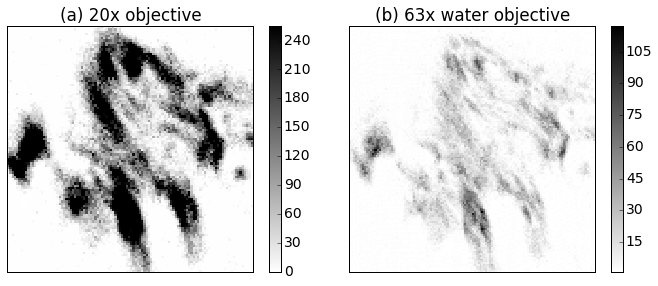
\includegraphics[width=\textwidth]{objectives}
\caption{Comparison of 20x dry objective to 63x water objective. Note that picture (a) have several pixels with maximum value (255). Settings for image (a) are PMT-gain of 700 Volt and scanning speed 400 Hz. Settings for image (b) are PMT-gain of 650 Volt and scanning speed 200 Hz.}
\label{fig:obj_comparison}
\end{figure}

Power equal 10\%, gain 60\% and offset 50\% for laser at 890 nm was found to create images taking use of whole 8 bit intensity range when PMT detector had gain of $\approx$ 600 Volt, but not the whole range of the HyD detector. Also some bright spots will make HyD detector shut down, giving large areas with zero value seen in figure \ref{fig:hyd}.

\begin{figure}
\centering
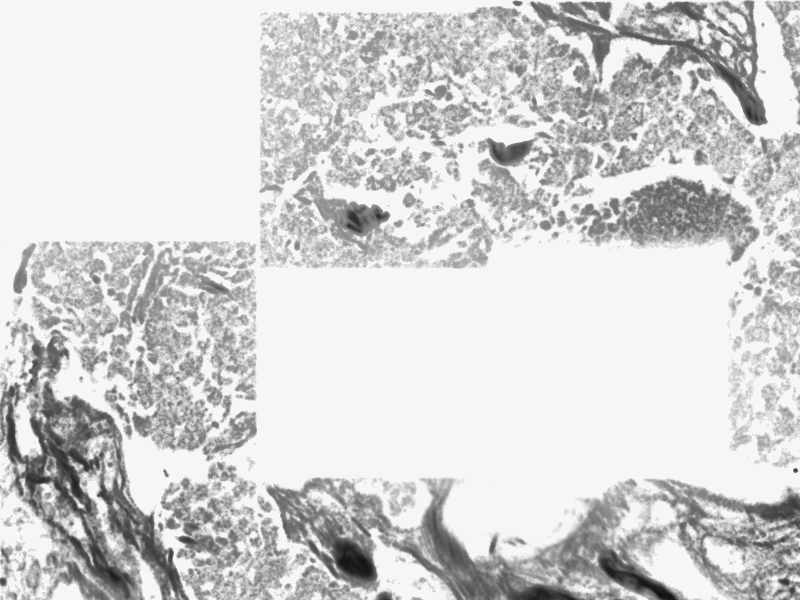
\includegraphics[width=0.5\textwidth]{hyd}
\caption{HyD detector have been shut off due to too strong signal. Image contrast is enhanced to improve visibility.}
\label{fig:hyd}
\end{figure}
 
Table \ref{tab:obj_time} show the minimum time for scanning an area of $\approx$ 1.2x1.2 mm$^2$ with pixel resolution below 200 nm. All times are given with scanning speed 600 Hz, which is the highest possible mirror oscillation frequency when using zoom factor 0.75 (minimum zoom factor possible).

\begin{table}[h]
\centering
\begin{tabular}{c c c c c c}
\hline
Objective & Zoom & Image size & Pixels & Number of images & Total time\\
\hline
20x & 0.97 & 600 $\mu$m & 4192 & 2x2 = 4 & 28 s \\
25x & 1.09 & 400 $\mu$m & 2048 & 3x3 = 9 & 31 s \\
63x & 0.92 & 200 $\mu$m & 1024 & 6x6 = 36 & 61 s \\
\hline
\end{tabular}
\caption{}
\label{tab:obj_time}
\end{table}


%
% TILESCAN VS WELLS
%
\section{Structured scan}
Figure \ref{fig:res_tilescan} show a merged tilescan. Note that several spots are uneven and that spots on left side are clipped of. Another defect is lower intensities at merging boarder, which is not easy to spot in the zoomed out figure \ref{fig:res_tilescan}, but is clearly seen in figure \ref{fig:spots}.

\begin{figure}[h]
\centering

\includegraphics[width=\textwidth]{result_tilescan}
\caption{Fluorescence tile scan with autofocus at regular intervals. Image is merged with Leica LAS AF.}
\label{fig:res_tilescan}
\end{figure}

Figure \ref{fig:single} shows an image taken with matrix scan. The image was merged from 5x5 scan fields, saving 11 images per well by omitting some of the sample.

\begin{figure}[h]
\centering
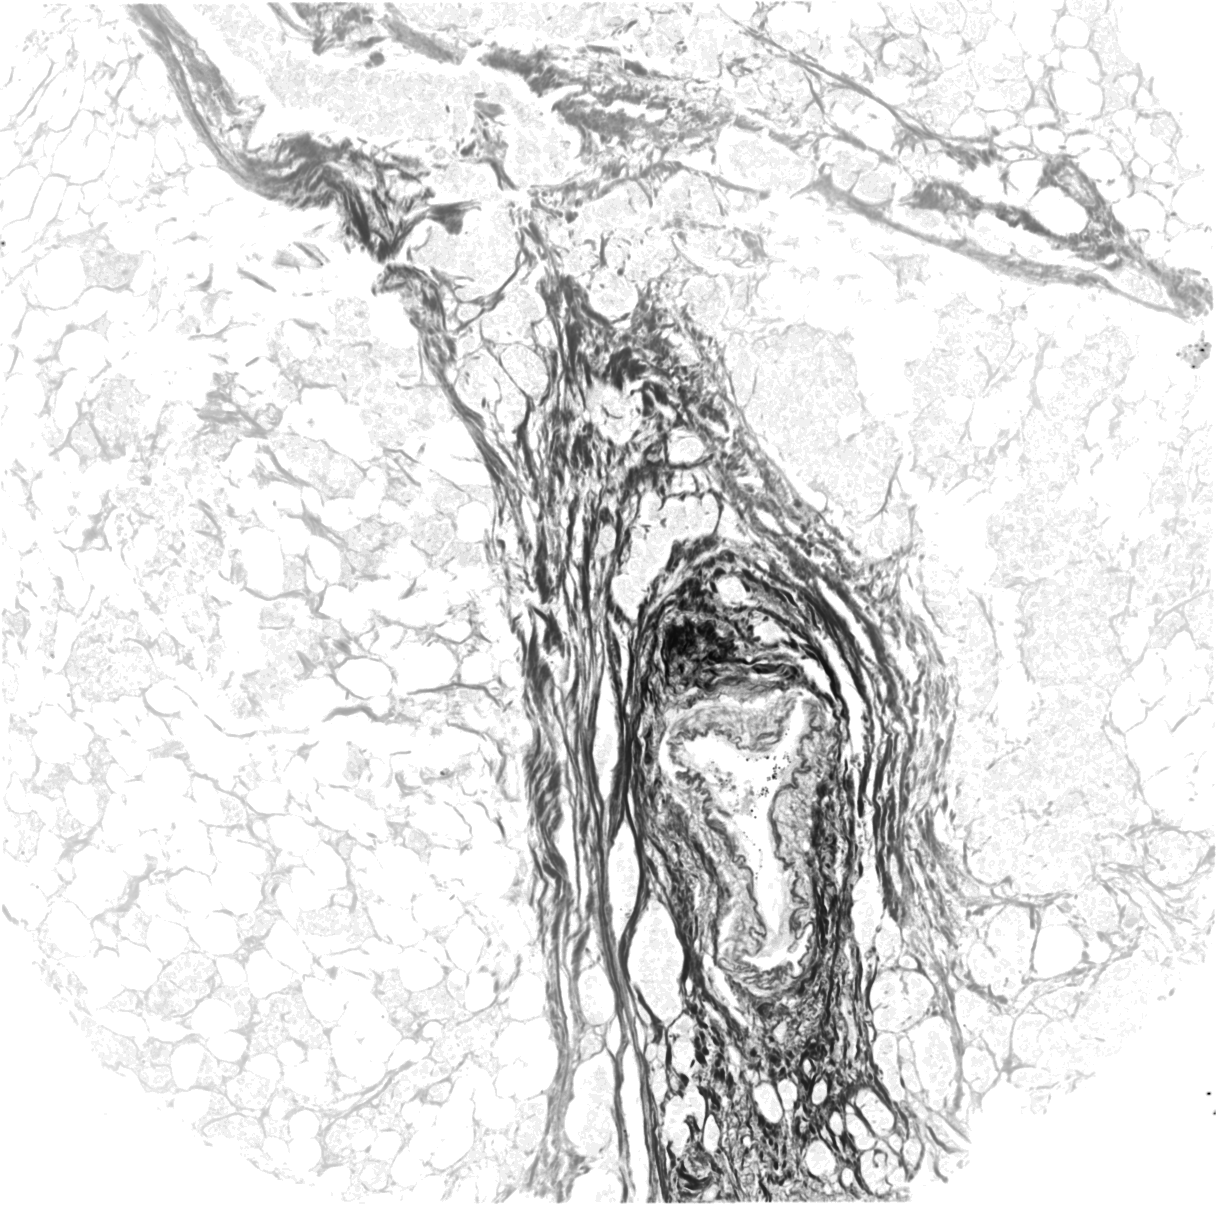
\includegraphics[width=0.33\textwidth]{single}
\caption{SHG image taken with matrix scan. Image have been merged with ImageJ and contrast enhanced with scikit-image. Area of image is 1136x1136 $\mu$m$^2$.}
\label{fig:single}
\end{figure}


%
% QUANTITATIVE
%
\section{Quantitative data}
Three samples have been picked out to illustrate the quantitative results. One image with fibers aligned in mostly one direction, one image with fibers in several directions and one image that seem anisotropic to human eye.

% HOG
% 
\subsection{Histogram of oriented gradients}
Figure \ref{fig:hist_grad_one}, \ref{fig:hist_grad_several} and \ref{fig:hist_grad_anisotropic} show histogram of angles calculated by the histogram of angles algorithm. Histogram of angles to all images have very strong response for angles 0, 45, 90 and 135, showing the weakness of calculating gradient on two dimensional data.

\begin{figure}[H]
\centering
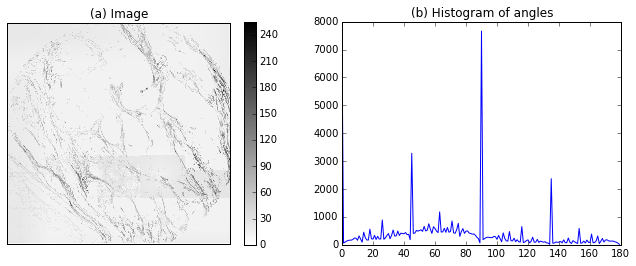
\includegraphics[width=0.8\textwidth]{hist_grad_one}
\caption{(a) Image of fibers in mostly one direction. (b) Histogram of angles calculated from gradient to image (a). A response between 40 and 90 is seen if one compare this histogram with figure \ref{fig:hist_grad_several} and \ref{fig:hist_grad_anisotropic}.}
\label{fig:hist_grad_one}
\end{figure}

\begin{figure}[H]
\centering
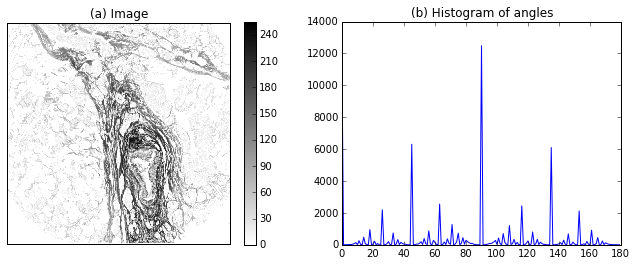
\includegraphics[width=0.8\textwidth]{hist_grad_several}
\caption{(a) Image with fibers in several directions. (b) Histogram of angles calculated from gradient to image (a). Histogram doesn't seem to contain any information about the direction of fibers in the image.}
\label{fig:hist_grad_several}
\end{figure}

\begin{figure}[H]
\centering
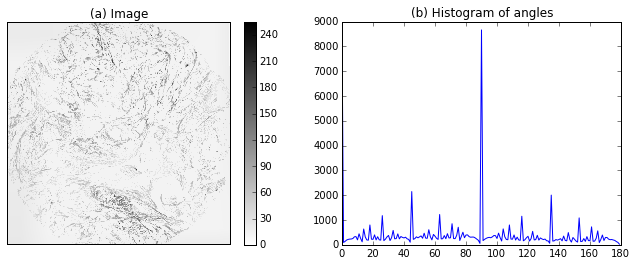
\includegraphics[width=0.8\textwidth]{hist_grad_anisotropic}
\caption{(a) Image which seems to be anisotropic to human eye. (b) Histogram of angles calculated from gradient of image (a). Histogram is very similar to figure \ref{fig:hist_grad_several} (b).}
\label{fig:hist_grad_anisotropic}
\end{figure}


% LINE
%
\subsection{Fourier transform}
\subsubsection{Line fit}
Figure \ref{fig:hist_line_one}, \ref{fig:hist_line_several} and \ref{fig:hist_line_anisotropic} show histogram of angles calculated by fitting a line in the Fourier spectrum. All images have similar response with high count of angles around 0 and 90 degrees.

\begin{figure}[h]
\centering
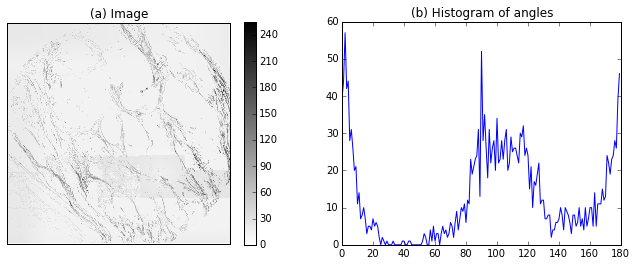
\includegraphics[width=0.8\textwidth]{hist_line_one}
\caption{(a) Image of fibers in mostly one direction. (b) Histogram of angles calculated by using line fit in Fourier spectrum.}
\label{fig:hist_line_one}
\end{figure}

\begin{figure}[h]
\centering
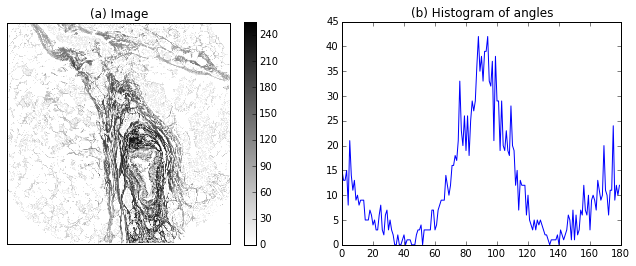
\includegraphics[width=0.8\textwidth]{hist_line_several}
\caption{(a) Image with fibers in several directions. (b) Histogram of angles calculated by using line fit in Fourier spectrum.}
\label{fig:hist_line_several}
\end{figure}

\begin{figure}[h]
\centering
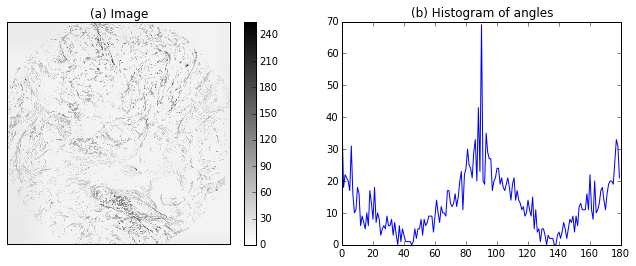
\includegraphics[width=0.8\textwidth]{hist_line_anisotropic}
\caption{(a) Image which seems to be anisotropic to human eye. (b) Histogram of angles calculated by using line fit in Fourier spectrum.}
\label{fig:hist_line_anisotropic}
\end{figure}


As figures \ref{fig:hist_line_one}, \ref{fig:hist_line_several} and \ref{fig:hist_line_anisotropic} show similar response, lines with a bad fit where discarded making figure \ref{fig:hist_line_one3}, \ref{fig:hist_line_several3} and \ref{fig:hist_line_anisotropic3}. Lines with correlation coefficient r$^2$ below 0.3 are discarded.


\begin{figure}[h]
\centering
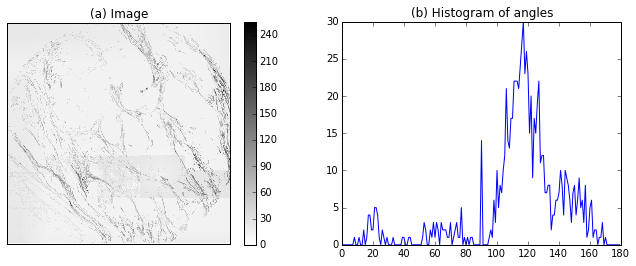
\includegraphics[width=0.8\textwidth]{hist_line_one3}
\caption{(a) Image of fibers in mostly one direction. (b) Histogram of angles calculated by using line fit in Fourier spectrum. Lines with r$^2$ < 0.3 are discarded. A clear response at about 120 degree is shown.}
\label{fig:hist_line_one3}
\end{figure}

\begin{figure}[h]
\centering
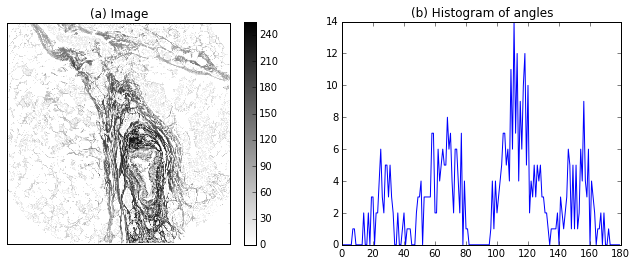
\includegraphics[width=0.8\textwidth]{hist_line_several3}
\caption{(a) Image with fibers in several directions. (b) Histogram of angles calculated by using line fit in Fourier spectrum. Lines with r$^2$ < 0.3 are discarded. Four clusters of angles are shown, $\approx$ 100-120 degree being the strongest response.}
\label{fig:hist_line_several3}
\end{figure}

\begin{figure}[h]
\centering
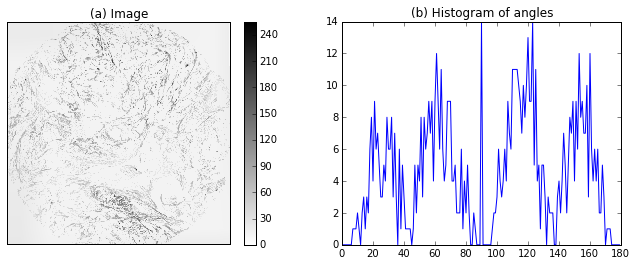
\includegraphics[width=0.8\textwidth]{hist_line_anisotropic3}
\caption{(a) Image which seems to be anisotropic to human eye. (b) Histogram of angles calculated by using line fit in Fourier spectrum. Lines with r$^2$ < 0.3 are discarded. Four roughly equal cluster of angles are shown.}
\label{fig:hist_line_anisotropic3}
\end{figure}


% SUM
%
\subsubsection{Sum of angles}
Figure \ref{fig:hist_sum_one}, \ref{fig:hist_sum_several} and \ref{fig:hist_sum_anisotropic} show histogram of angles calculated by summing up angles of top intensity pixels in Fourier spectrum.

\begin{figure}[h]
\centering
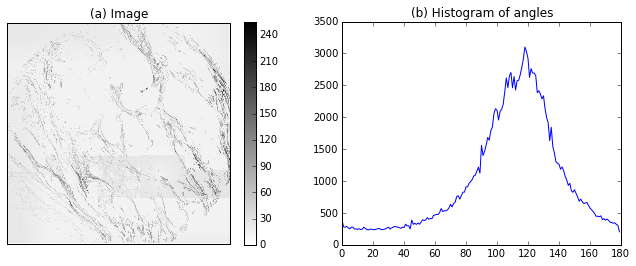
\includegraphics[width=0.8\textwidth]{hist_sum_one}
\caption{(a) Image of fibers in mostly one direction. (b) Histogram of angles calculated by summing up the angle of top intensity pixels in Fourier spectrum. Histogram have a peak at $\approx$ 125 degree with $\approx$ 40 degrees width.}
\label{fig:hist_sum_one}
\end{figure}

\begin{figure}[h]
\centering
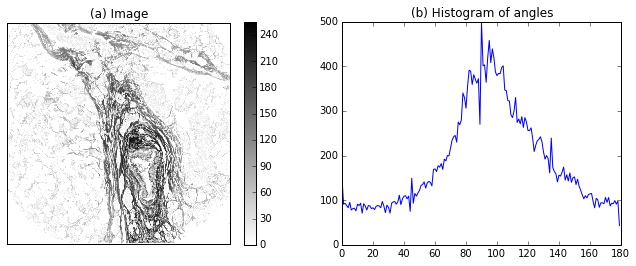
\includegraphics[width=0.8\textwidth]{hist_sum_several}
\caption{(a) Image with fibers in several directions. (b) Histogram of angles calculated by summing up the angle of top intensity pixels in Fourier spectrum.
Histogram have a peak at $\approx$ 95 degree with $\approx$ 50 degrees width.}
\label{fig:hist_sum_several}
\end{figure}

\begin{figure}[h]
\centering
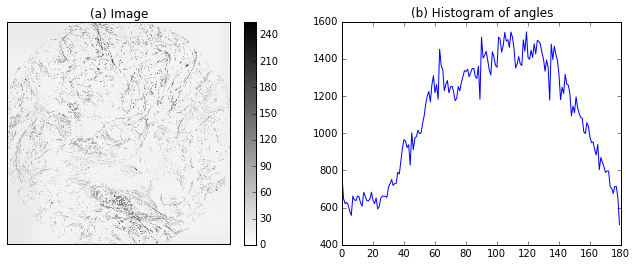
\includegraphics[width=0.8\textwidth]{hist_sum_anisotropic}
\caption{(a) Image which seems to be anisotropic to human eye. (b) Histogram of angles calculated by summing up the angle of top intensity pixels in Fourier spectrum. Histogram have a high count of angles from $\approx$ 40 to 160 degrees, making a broad peak.}
\label{fig:hist_sum_anisotropic}
\end{figure}